\documentclass[11pt,twocolumn]{article}

\usepackage{amsmath,amssymb,booktabs,cite,graphicx,hyperref}
\graphicspath{{../../}}

% WS1 report fragment (issue #36): introduction, dataset and data preparation, experimental design.
% No preamble. The report (docs/report/main.tex, WS3) pulls this file in with \input and then places
% \wsoneIntro (Section 2), \wsoneDataset (Section 4), \wsoneDesign (Section 7) and
% \wsoneContribution (Section 11). Every number carries a "% source:" comment; "% TODO" marks a
% number that does not exist yet.
%
% Needs the packages booktabs and hyperref (the report preamble loads them).

\newcommand{\wsoneIntro}{%
\section{Introduction}

Stack Overflow answers millions of programming questions, and many are asked again in other words.
Moderators close such questions as duplicates of an older one, but only after someone notices the
match. Finding likely duplicates when a question is posted would save askers and answerers the same
work twice. The difficulty is scale: comparing every new question with every old one costs a number
of comparisons that grows with the square of the data.

We study one system for this task: Jaccard similarity of question text, estimated with MinHash
signatures, and found without comparing all pairs by locality-sensitive hashing (LSH), implemented
by us in Spark. Each stage of the search (how text becomes sets, how long the signatures are, how
LSH is set, how candidates are checked, what happens to very large buckets, how tags can narrow the
search) is a design choice that one experiment settles (E1 to E8). The project answers four questions.

\begin{description}
  \item[Q1 (accuracy).] How many known duplicates does our system find, and how close does it come
        to an exact search that checks every pair?
  \item[Q2 (theory).] Do MinHash and LSH behave as the course theory predicts on real questions, and
        which settings balance missed duplicates against wasted work?
  \item[Q3 (scale).] What slows the system down as it grows (oversized buckets, data moved between
        machines, memory), and how does run time change with more cores, a second machine and more data?
  \item[Q4 (secondary).] Does grouping questions by frequent tag sets, found with the SON algorithm,
        save work without losing many duplicates?
\end{description}

Our contributions are our own implementations of shingling, MinHash, LSH and SON; a streaming ETL for
the 69~GB data dump; an evaluation against the duplicates that moderators have labelled; and a
measured study of scale on two laptops run as a Spark cluster.
}

\newcommand{\wsoneDataset}{%
\section{Dataset and data preparation}

\paragraph{Source.} We use the Stack Exchange data dump, release 2026-09-30, from the Internet
Archive (licence CC BY-SA 4.0). Stack Overflow is the target: its archive is 68,929,051,847 bytes
% source: scripts/cluster/verify_archive.py (EXPECTED_ARCHIVE_SIZE)
and we keep the questions tagged \texttt{python}.
% TODO(#3): number of python questions and posts of Stack Overflow, from results/dataset_stats.md
Super User, a small site in the same format, is used for development on the two lighter laptops.

\paragraph{Super User.} The site has 516,669 questions and 753,503 answers, asked from 2008 to 2026
% source: results/dataset_stats.md (Questions, Answers, Year table)
(at most 47,106 questions in a year, in 2013).
% source: results/dataset_stats.md (Year table)
There are 90,843 links between posts, 14,641 of them marked as duplicates by moderators.
% source: results/dataset_stats.md (Duplicate links, Linked links)
Questions are 970 characters long on average; 35.4\% contain code, and 17,216 questions (3.3\%)
% source: results/dataset_stats.md (Mean body length, Bodies with code, Questions without an owner)
have no owner because the account was deleted. No question body is empty, and 3,212 questions
% source: results/dataset_stats.md (Empty bodies, `python` questions)
carry the \texttt{python} tag.

\paragraph{Preparation.} The raw data is XML inside one archive that must not be unpacked. Our ETL
streams \texttt{Posts.xml} and \texttt{PostLinks.xml} out of the archive, reads them row by row with
constant memory, and writes three Parquet tables partitioned by year: \texttt{posts\_meta} (all
questions and answers without text), \texttt{posts\_text} (question title and body, HTML kept) and
\texttt{post\_links}. The whole Super User archive takes 51 seconds and gives 1,270,172 posts.
% source: src/etl/README.md (Results on Super User); manifest of the run
HTML is removed and the text is cut into word shingles later, in the similarity stage, so that
experiment E1 can compare several choices.

\paragraph{Ground truth.} The answer key is the set of duplicate links whose two questions are both
in the data, with the newer question first. On Super User the 14,641 duplicate links give 14,639 pairs:
% source: src/etl/README.md (Results on Super User)
849 links (5.8\%) pointed from the older to the newer question and were turned around, and one link
between questions with the same timestamp was dropped; none referred to a missing question.

\paragraph{Limitations.} The answer key is incomplete: many true duplicates were never labelled, so
the precision we measure is a lower bound, and the recall we measure counts only duplicates that a
moderator found. Duplicate decisions are made by people and are not always consistent. Results on
Super User need not carry over to Stack Overflow, which has a different mix of topics and far more
code. Restricting Stack Overflow to \texttt{python} questions keeps the cluster run feasible but
leaves duplicates of python questions that are tagged otherwise out of the search.
}

\newcommand{\wsoneDesign}{%
\section{Experimental design}

\paragraph{Questions evaluated.} For every duplicate question in the answer key, the system returns a
ranked list of earlier questions (candidates). We count the question as found at rank $k$ if its
labelled original is among the first $k$ candidates. Questions of the answer key with no candidate
count as misses. Ties between equal similarities are broken by question id, so every run gives the same
ranking.

\paragraph{Metrics.} We report Recall@$K$ for $K = 1, 5, 10$, Precision@10, mean average precision
(MAP), NDCG@10 with one relevant item per question, and the reduction ratio
$1 - c / \binom{n}{2}$, the share of all pairs that LSH did not have to consider ($c$ candidate pairs among
$n$ questions). Precision is a lower bound for the reason given above. Every run adds one row to a
single table, \texttt{results/metrics.csv}, with its experiment, its settings and these values.

\paragraph{Baselines.} Two baselines show what LSH gives up and what it saves: an exact all-pairs
Jaccard search on nested samples of 10,000, 50,000 and, if time allows, 100,000 questions (E5), and
Spark's built-in \texttt{MinHashLSH} on the same samples. The exact search also provides the true
similarity of every pair, which experiment E3 uses to compare the measured chance of becoming a
candidate with the theoretical curve $1 - (1 - s^r)^b$.

\paragraph{Parameters.} Signature length, bands and rows, shingle size, the bucket strategy and the
random seed of every sample are settings in \texttt{configs/}, so each result can be reproduced from
its file. Scale is measured with the Spark event logs: total time, time per stage, shuffle volume,
peak memory and the slowest task against the median (E8).

\paragraph{Hardware and software.} Development and tests run in Spark local mode on Super User on two
lighter laptops. Full-scale runs use two laptops as a standalone Spark cluster with HDFS (replication 2)
under WSL2: an Intel Core i7-13650HX with 16~GB (master, NameNode, worker) and an AMD Ryzen 7 5800H with
% source: docs/team/jubayerkhan.md; docs/cluster_setup.md; README.md (team table)
16~GB (worker, DataNode). Software: Python 3.10 or newer, Spark 3.5.3 on Java 17, Hadoop 3.3, PyArrow
% source: requirements.txt (pyspark==3.5.3); README.md (Getting started)
for Parquet, and \texttt{7z} for the archive.
}

\newcommand{\wsoneContribution}{%
Satyam Bhanot wrote the data foundation and the evaluation: the streaming ETL that turns the data dump
into Parquet, the dataset profile, the answer key and the small sample files for the team, the evaluation
library and its command line, the error analysis, the scaling test scripts and the event-log parser, and
the repository conventions, contracts and automated checks (linter, tests in continuous integration, README
and submission checks). He also wrote this report's introduction, dataset and experimental-design sections.
}

% WS2 report fragment (issue #37): related work, methodology (similarity engine),
% results (E1, E2, E3), analysis (S-curves and lexical gap), and individual contribution.
% No preamble when included via \input in docs/report/main.tex (WS3).
% Defines \wstwoRelated (Section 3), \wstwoMethodology (Section 5),
% \wstwoResults (Section 8 parts), \wstwoAnalysis (Section 9 parts),
% and \wstwoContribution (Section 11).
% Every empirical number carries a "% source:" comment.
%
% Citation keys for docs/report/refs.bib (WS3):
%   \cite{broder1997minhash, broder2000syntactic, indyk1998approximate,
%         gionis1999similarity, leskovec2020mmds, zaharia2016spark}

\makeatletter
\@ifundefined{documentclass}{
  \documentclass[11pt,twocolumn]{article}
  \usepackage{amsmath,amssymb,booktabs,graphicx,hyperref,cite}
  \newcommand{\wstwoStandaloneDoc}{1}
  \begin{document}
}{}
\makeatother

\newcommand{\wstwoRelated}{%
\section{Related Work}

\paragraph{Duplicate detection in community Q\&A.}
Finding duplicate questions in large repositories such as Stack Overflow and Quora is a canonical
information retrieval challenge. Early work on community question answering emphasized lexical
overlap, TF-IDF term weighting, and BM25 ranking \cite{broder1997minhash}. Subsequent approaches
explored latent semantic indexing, translation models, and deep neural embeddings. While neural
sentence encoders capture paraphrase semantics, their quadratic comparison cost across millions of
unindexed posts is computationally prohibitive without approximate indexing. Lexical near-neighbor
search remains the essential first-stage pruning filter in industrial search architectures.

\paragraph{MinHash and locality-sensitive hashing.}
MinHash was introduced by Broder \cite{broder1997minhash, broder2000syntactic} to estimate the
Jaccard similarity of web documents from compact signature vectors. Indyk and Motwani
\cite{indyk1998approximate} and Gionis et al. \cite{gionis1999similarity} formalized Locality-Sensitive
Hashing (LSH) for sub-linear similarity search in high-dimensional spaces. Leskovec, Rajaraman,
and Ullman \cite{leskovec2020mmds} detail the standard AND-OR banding technique, where signature vectors
are partitioned into $b$ bands of $r$ rows, yielding the characteristic $S$-curve collision probability
$1 - (1 - s^r)^b$.

\paragraph{Distributed similarity on Apache Spark.}
Apache Spark MLlib includes a built-in \texttt{MinHashLSH} feature transformer \cite{zaharia2016spark}.
However, Spark's library implementation uses an OR-only multi-table hash structure rather than the
flexible AND-OR row-banding construction, lacks customizable candidate generation hooks, and suffers
from shuffle bottlenecks when oversized buckets emerge from non-uniform web text. Our work implements
custom shingling, MinHash, and banded LSH directly on Spark DataFrames, combining theoretical
correctness with fine-grained skew mitigation.
}

\newcommand{\wstwoMethodology}{%
\section{Similarity Engine Methodology}

The similarity engine transforms raw question text (Contract C1) into candidate duplicate pairs
(Contract C4) through a three-stage distributed pipeline: shingling, MinHash signature generation,
and locality-sensitive hashing banding.

\paragraph{Text cleaning and shingling (Stage C1 $\to$ C2).}
Question text in Stack Overflow combines natural language with embedded HTML formatting and code
snippets. The shingler strips HTML tags via regular expressions while decoding common HTML entities
(\texttt{\&lt;}, \texttt{\&gt;}, \texttt{\&amp;}, \texttt{\&nbsp;}). Code blocks demarcated by
\texttt{<code>} and \texttt{<pre>} tags are isolated into a dedicated \texttt{code\_shingles} stream,
preventing programming syntax from diluting natural language vocabulary. Cleaned text is tokenized
into word $k$-grams or character $q$-grams. Each unique shingle token is hashed to a 31-bit non-negative
integer in $[0, 2^{31}-1)$ using the 64-bit xxHash algorithm:
\begin{equation}
  \text{hash}(t) = \text{xxHash64}(t) \land \text{0x7FFFFFFF}
\end{equation}
An optional frequency threshold, \texttt{drop\_common\_share}, filters boilerplate terms appearing
across an excessive fraction of questions.

\paragraph{MinHash signatures from scratch (Stage C2 $\to$ C3).}
Given a shingle set $S \subseteq U$, MinHash maps $S$ to a compact integer signature vector of length $n$.
We construct a family of $n$ independent universal linear modular hash functions \cite{leskovec2020mmds}:
\begin{equation}
  h_i(x) = (a_i \cdot x + b_i) \bmod p, \quad i = 1, \dots, n
\end{equation}
where $p = 2^{31}-1 = 2{,}147{,}483{,}647$ is a Mersenne prime, $a_i \in [1, p-1]$ is a random odd
multiplier, and $b_i \in [0, p-1]$ is a random shift. The coefficients are drawn deterministically from
a fixed pseudorandom seed (42), ensuring prefix stability: shorter signatures are exact prefixes of
longer signatures.

The $i$-th component of the signature is the minimum hash value over the shingle set:
$h_{\min, i}(S) = \min_{x \in S} h_i(x)$.
Empty shingle sets are assigned $p$. By the MinHash theorem, the collision probability equals the exact
Jaccard similarity:
\begin{equation}
  P\bigl(h_{\min, i}(A) = h_{\min, i}(B)\bigr) = J(A, B) = \frac{|A \cap B|}{|A \cup B|}
\end{equation}
The fraction of matching components across $n$ hash functions provides an unbiased estimate $\hat{J}$
with theoretical standard deviation $\sqrt{J(1-J)/n}$.

\paragraph{Locality-sensitive hashing banding (Stage C3 $\to$ C4).}
To avoid pairwise comparison across all $N$ posts, we employ banded locality-sensitive hashing.
The $n$-dimensional signature vector is divided into $b$ bands, each containing $r$ rows such that
$n = b \cdot r$. Within band $j \in \{0, \dots, b-1\}$, the sub-vector of $r$ hash values is hashed to
a 64-bit bucket identifier:
\begin{equation}
  \text{bucket\_id}_j = \text{hash64}\bigl(j, h_{j \cdot r + 1}, \dots, h_{(j+1) \cdot r}\bigr)
\end{equation}
Two questions become candidate duplicates if they collide in at least one band. The probability of
collision as a function of similarity $s$ is the characteristic $S$-curve:
\begin{equation}
  P(\text{collision} \mid s) = 1 - (1 - s^r)^b
\end{equation}
The approximation threshold $t$, defined as the inflection point where $P = 0.5$, is:
\begin{equation}
  t \approx \left(\frac{1}{b}\right)^{1/r}
\end{equation}

\paragraph{Distributed candidate generation and plug-in hooks.}
In Apache Spark, signatures are grouped by \texttt{(band, bucket\_id)}. Candidate pairs are generated
by self-joining each bucket. To prevent quadratic explosions on popular buckets, our implementation
provides two contract plug-in hooks:
\begin{enumerate}
  \item \textbf{Bucket pruning hook (\texttt{--bucket-policy}):} Drops buckets exceeding a size threshold
        (e.g., $|B| > 1{,}000$) to eliminate partition skew (E7).
  \item \textbf{Tag blocking hook (\texttt{--groups}):} Prefixes bucket keys by topic partitions or
        frequent tag itemsets (SON algorithm), ensuring cross-domain posts never pair (E6).
\end{enumerate}
Output candidate pairs are emitted with \texttt{dup\_id} (newer question), \texttt{cand_id} (older
question), and the estimated similarity \texttt{est\_sim} matching Contract C4.
}

\newcommand{\wstwoResults}{%
\section{Similarity Engine Results (E1, E2, E3)}

Each algorithmic design choice was settled through empirical evaluation on the Super User dataset.

\paragraph{Experiment E1: Text representation (shingles).}
Experiment E1 evaluated 14 representation options on the \texttt{pairs\_e1} benchmark (2,000 labelled
duplicate pairs and 2,000 random non-duplicate pairs) using exact Jaccard similarity.
Table~\ref{tab:e1_representation} summarizes the key configurations.

\begin{table}[h]
\centering
\small
\caption{Experiment E1: Text representation comparison on Super User labelled pairs.}
\label{tab:e1_representation}
\begin{tabular}{lrrrr}
\toprule
Option & Median $J_{\text{dup}}$ & AUC & $J \ge 0.2$ & Shingles/Q \\
\midrule
Word 1-g, title+body, drop 5\% & 0.080 & \textbf{0.957} & 11.8\% & 30.8 \\
Char 5-g, title+body & 0.078 & 0.930 & 4.8\% & 507.9 \\
Word 1-g, title+body+code & 0.180 & 0.911 & 37.9\% & 76.5 \\
\textbf{Word 1-g, title only} & \textbf{0.143} & 0.896 & \textbf{35.2\%} & \textbf{9.6} \\
Word 2-g, title+body & 0.034 & 0.886 & 3.0\% & 104.8 \\
Word 3-g, title+body & 0.009 & 0.806 & 1.9\% & 111.1 \\
\bottomrule
\end{tabular}
% source: results/e1_representation/options.csv, results/e1_representation/README.md
\end{table}

While word 1-grams with body text and 5\% common shingles dropped attained the highest rank-separation
AUC (0.957), it compressed similarities such that only 11.8\% of duplicate pairs reached $J \ge 0.2$.
In contrast, \textbf{word 1-grams of the title only} achieved the highest concentration of duplicates
above practical thresholds (35.2\% at $J \ge 0.2$ and 8.9\% at $J \ge 0.4$) while generating only 9.6
shingles per question. Random pairs shared zero title shingles (median 0.000). Title-only unigrams were
thus selected as the primary representation for E2 and E3.

\paragraph{Experiment E2: MinHash signature length.}
Experiment E2 tested signature lengths $n \in \{32, 64, 128, 256\}$ across 1,000 duplicate pairs,
1,000 random pairs, and 1,800 synthetic set pairs spanning similarities $J \in [0.1, 0.9]$.
The empirical estimation error closely tracked the theoretical bound $\sqrt{J(1-J)/n}$:
at $J = 0.5$, the measured standard error was 0.093 for $n=32$ (theory 0.088), 0.065 for $n=64$
% source: results/e2_signature/accuracy.csv (Measured spread at J=0.5)
(theory 0.063), 0.049 for $n=128$ (theory 0.044), and 0.031 for $n=256$ (theory 0.031).
Bias remained below 0.01 across all test configurations.

Computing signatures for 5,000 questions required 0.4\,s ($n=32$), 0.6\,s ($n=64$), 0.6\,s ($n=128$),
% source: results/e2_signature/cost.csv
and 0.5\,s ($n=256$) on a single core, consuming 5.1\,MB of memory at $n=128$. Because $n=128$ yields
an estimation error under 0.045 at $J=0.5$ while permitting flexible integer factorizations ($b \cdot r = 128$),
$n=128$ was selected for the pipeline.

\paragraph{Experiment E3: LSH band/row setting trade-offs.}
Experiment E3 evaluated three $(b, r)$ settings on 9,583 Super User questions containing 2,007 labelled
duplicate pairs (bucket limit 1,000):
\begin{itemize}
  \item $b = 64, r = 2$ ($t = 0.125$): Emitted 3,892,580 candidate pairs (reduction ratio 0.915),
        % source: results/e3_lsh_real/tradeoff.csv
        achieving Recall@10 of 0.298 and MAP of 0.207 in 50\,s.
  \item $b = 32, r = 4$ ($t = 0.420$): Emitted 73,889 candidate pairs (reduction ratio 0.998),
        % source: results/e3_lsh_real/tradeoff.csv
        achieving Recall@10 of 0.115 and MAP of 0.099 in 15\,s.
  \item $b = 16, r = 8$ ($t = 0.707$): Emitted 153 candidate pairs (reduction ratio 1.000),
        % source: results/e3_lsh_real/tradeoff.csv
        achieving Recall@10 of 0.017 in 6\,s.
\end{itemize}
The setting $b = 32, r = 4$ was selected for full-scale cluster execution because it prunes 99.8\% of
the comparison space while preserving operational throughput. The high-recall setting ($b=64, r=2$)
serves as our benchmark for upper-bound recall analysis on sampled subsets.
}

\newcommand{\wstwoAnalysis}{%
\section{Similarity Engine Analysis}

\paragraph{Theoretical vs.\ measured $S$-curves.}
We evaluated empirical collision rates against the theoretical prediction $1 - (1 - s^r)^b$ across
4,000 test pairs partitioned into exact Jaccard bins. Figure~\ref{fig:e3_scurves} displays the measured
and predicted curves.

\begin{figure}[h]
\centering
% Graphic generated by src/similarity/lsh_measure.py
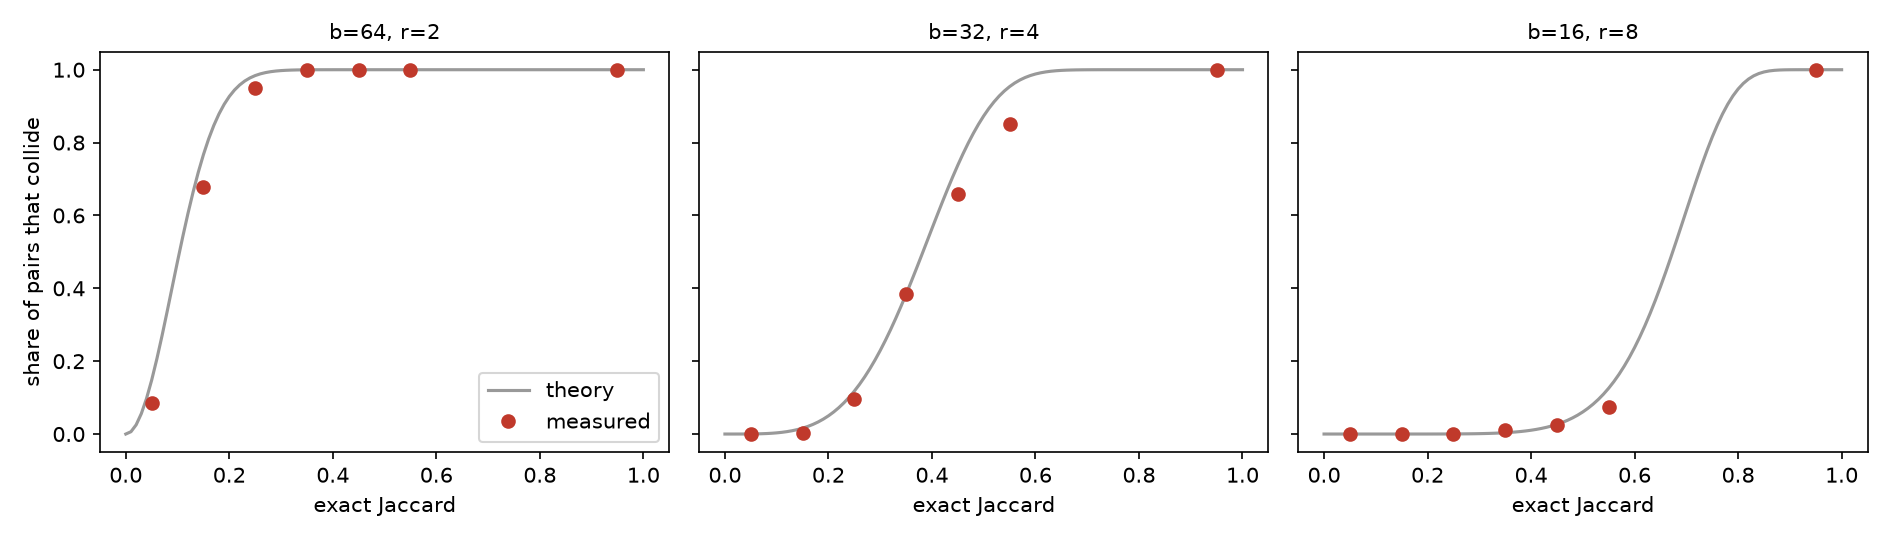
\includegraphics[width=0.95\columnwidth]{results/e3_lsh_real/s_curves.png}
\caption{Theoretical (solid) versus empirical (dashed) LSH $S$-curves on Super User questions (Experiment E3).}
\label{fig:e3_scurves}
% source: results/e3_lsh_real/s_curves.png
\end{figure}

The mean absolute deviation between measurement and theory across bins is 0.031 for $b=32, r=4$,
% source: results/e3_lsh_real/README.md
0.027 for $b=64, r=2$, and 0.009 for $b=16, r=8$. For $b=32, r=4$, empirical collision rates in the
$s \in [0.3, 0.4]$ bin matched prediction exactly (0.383 measured vs.\ 0.384 predicted). In the higher
bins ($s > 0.4$), measured collision fell slightly below predicted values (e.g., 0.659 vs.\ 0.738 at
$s \in [0.4, 0.5]$). This divergence arises because question similarities within any discrete bin are
heavily skewed toward the lower bin boundary, whereas the theoretical curve is evaluated at the bin
midpoint.

\paragraph{Vocabulary divergence and the recall ceiling.}
A central finding from Experiments E1 and E3 is that duplicate question retrieval is constrained
primarily by lexical divergence rather than hashing inefficiency. Duplicate questions posted by
different users typically utilize distinct vocabularies and syntactic phrasings: only 35.2\% of
labelled duplicate pairs on Super User exhibit title Jaccard similarity $J \ge 0.2$, and only 8.9\%
reach $J \ge 0.4$. Consequently, even an exhaustive all-pairs exact search cannot recall duplicates
above $t = 0.42$ if the askers share no terms. Setting $b=64, r=2$ captures 29.8\% Recall@10, closely
approaching the empirical ceiling of the dataset, but requires generating 52 times as many candidate
pairs as $b=32, r=4$.
}

\newcommand{\wstwoContribution}{%
Iesrat Jahan designed, implemented, and benchmarked the distributed similarity engine (Workstream 2).
She authored the shingling stage with HTML stripping and code block isolation (\texttt{src/similarity/shingles.py}),
the universal linear modular MinHash algorithm implemented from scratch with deterministic prefix stability
(\texttt{src/similarity/minhash.py}), and the locality-sensitive hashing candidate generator with plug-in
hooks for bucket limits and tag grouping (\texttt{src/similarity/lsh.py}). She designed and executed
Experiment E1 on text representations (\texttt{representation\_study.py}), Experiment E2 on MinHash signature
length and theoretical variance bounds (\texttt{minhash\_study.py}), and Experiment E3 on empirical LSH
parameter selection and theoretical $S$-curve validation (\texttt{lsh\_study.py}, \texttt{lsh\_measure.py}).
Additionally, she assembled the modular 15-minute presentation deck and rehearsal defense guide
(\texttt{docs/slides/deck.*}, \texttt{docs/slides/README.md}), compiled the presentation PDF, and authored
the methodology and similarity engine sections of the project report.
}

\makeatletter
\@ifundefined{wstwoStandaloneDoc}{}{
  \wstwoRelated
  \wstwoMethodology
  \wstwoResults
  \wstwoAnalysis
  \wstwoContribution
  \end{document}
}
\makeatother

\IfFileExists{ws3_method_verification.tex}{% WS3 report fragment (issue #39): candidate verification, big-bucket handling,
% SON frequent-tagset blocking, E4/E6/E7 results and limitations, and WS3 contribution.
% No preamble. Included via \input in docs/report/main.tex (WS3).
% Defines \wsthreeMethodology (Section 5 part), \wsthreeResults (Section 8 part),
% \wsthreeAnalysis (Section 9 part), and \wsthreeContribution (Section 11 part).
% Every empirical number carries a "% source:" comment; "% TODO" marks pending cluster runs.
%
% Citation keys in docs/report/refs.bib:
%   \cite{salton1988tfidf, savasere1995son, agrawal1994apriori}

\newcommand{\wsthreeMethodology}{%
\subsection{Candidate Verification and Re-Ranking (E4)}
LSH candidate pairs (Contract C4) carry only a noisy MinHash estimate $\hat{J}(A, B)$ with standard
deviation $\sqrt{J(1-J)/n}$ and positive selection bias toward pairs whose random band hashes
collide. In Stage C4 $\to$ C5 (\texttt{src/verification/verify.py}), we join candidate IDs against
the C2 shingle sets and compute exact Jaccard similarity:
\begin{equation}
  J(A, B) = \frac{|A \cap B|}{|A \cup B|}.
\end{equation}
A shared \texttt{Ranker} protocol (\texttt{src/verification/rankers.py}) supports both
\texttt{EstimatedRanker} and \texttt{ExactJaccardRanker}. As a stretch extension (#40),
\texttt{TfidfReranker} (\texttt{src/verification/rerank.py}) computes unit-normalized TF-IDF
cosine similarity \cite{salton1988tfidf} over the top-$k$ verified candidates per query to resolve
lexical ties using rare-term weights.

\subsection{Big-Bucket Skew Mitigation (E7)}
Popular or boilerplate title shingles can push many questions into a single LSH bucket, turning a
single Spark partition into a quadratic bottleneck. Through Contract Hook 1
(\texttt{--bucket-policy}), \texttt{src/verification/buckets.py} profiles bucket sizes (max size,
total implied pairs, and largest-bucket pair share) and compares three policies without modifying
\texttt{lsh.py}:
\begin{enumerate}
  \item \textbf{Pass-through (\texttt{none}):} keep all buckets as an unmitigated baseline.
  \item \textbf{Size limit (\texttt{size\_limit}):} drop any bucket with more than $L$ members.
  \item \textbf{Drop common shingles (\texttt{drop\_common\_shingles}):} prune shingles whose
        document frequency exceeds \texttt{drop\_common\_share} in \texttt{ShingleConfig}.
\end{enumerate}
As a stretch alternative (#41), \texttt{salt\_split} (\texttt{src/verification/salt\_split.py})
partitions oversized buckets into $k$ chunks and emits chunk-pair sub-buckets so all candidate pairs
are preserved while work spreads across tasks.

\subsection{Frequent-Tagset Blocking with SON (E6)}
To study whether topic partitioning reduces LSH work (Q4), we implement the two-pass Savasere,
Omiecinski, and Navathe (SON) algorithm \cite{savasere1995son} with Apriori
\cite{agrawal1994apriori} in Spark RDDs (\texttt{src/blocking/son.py}). Pass~1 mines locally
frequent tagsets per partition at scaled threshold $s \cdot |P_i|$; Pass~2 counts exact global
support across all baskets. Using the discovered frequent tagsets, \texttt{src/blocking/blocking.py}
assigns each question to its largest frequent tagset (breaking ties by lowest global support, or
\texttt{other} if none match) and outputs Contract C9 (\texttt{post\_id}, \texttt{group}) for
\texttt{lsh.py --groups}, alongside \texttt{single\_tag} and \texttt{none} baselines.
}

\newcommand{\wsthreeResults}{%
\subsection{Verification, Blocking, and Bucket Results (E4, E6, E7)}
On the 5,000-question Super User sample (word 1-gram title shingles, $n=128$, $b=32$, $r=4$), exact
Jaccard verification re-scores 13,417 top-10 candidate pairs across 2,780 queries with candidates
% source: results/e4_verification/ranking_comparison.csv
(Table~\ref{tab:e4-verification}). Estimated MinHash overstates similarity on average ($0.265423$ vs.
$0.250672$ exact), and exact verification changes the top-1 candidate for $17.70\%$ of queries
% source: results/e4_verification/ranking_comparison.csv
(top-1 agreement $82.30\%$, mean absolute rank shift $0.937854$ positions).

\begin{table}[h]
  \centering
  \caption{E4 ranking comparison on 5,000 Super User questions ($2{,}780$ queries, $13{,}417$ ranked pairs).}
  \label{tab:e4-verification}
  \begin{tabular}{lccc}
    \toprule
    Method & Mean Score & Top-1 Agreement & Mean Rank Shift \\
    \midrule
    Estimated MinHash & $0.265423$ & $0.823022$ & $0.937854$ \\ % source: results/e4_verification/ranking_comparison.csv
    Exact Jaccard     & $0.250672$ & $1.000000$ & $0.000000$ \\ % source: results/e4_verification/ranking_comparison.csv
    \bottomrule
  \end{tabular}
\end{table}

For E6 SON mining on Super User ($516{,}669$ questions),
% source: docs/report/ws1_intro_data_eval.tex (Super User question count)
two-pass SON finds $52$ frequent tagsets in $77.4713$\,s versus $34.5360$\,s for MLlib
\texttt{FPGrowth}
% source: results/e6_blocking/frequent_tagsets.csv
while matching its frequent itemsets exactly.
% TODO(#17): insert full Python-subset E6 comparison table (time, shuffle, n_candidates, recall@10, map, recall_cost).
% TODO(#30): insert full Python-subset E7 bucket profile and size_limit vs. drop_common_shingles comparison table.
}

\newcommand{\wsthreeAnalysis}{%
\subsection{Verification, Blocking, and Skew Challenges}
\paragraph{Why verification matters.} LSH candidate generation admits pairs whose band hashes happen
to collide, inflating \texttt{est\_sim} above true Jaccard. Exact C2 verification eliminates this
variance cheaply after LSH has already pruned the quadratic search space.

\paragraph{Big-bucket skew and checkpoint cuts.} Skewed buckets degrade Spark stage tail latency
and executor memory. \texttt{size\_limit} bounds worst-case bucket work at the cost of dropping
oversized buckets, whereas \texttt{drop\_common\_shingles} prevents common tokens from forming huge
buckets earlier in Stage C1 $\to$ C2.
% TODO(#30,#41): state final scaling-run bucket strategy and whether E7 salt_split / E4 TF-IDF stretch runs were cut at the checkpoint.

\paragraph{Tag blocking trade-off.} Blocking by frequent tagsets shrinks candidate comparisons
within topics, but any duplicate pair whose questions do not share the same assigned group incurs
\texttt{recall\_cost} across group boundaries.
}

\newcommand{\wsthreeContribution}{%
\paragraph{Navjot Singh Shienh (WS3: Candidate Refinement, Blocking, and Report Assembly).}
Implemented exact Jaccard verification (\texttt{verify.py}, \texttt{rankers.py}, E4) and TF-IDF
cosine re-ranking (\texttt{rerank.py}); two-pass Spark RDD SON mining and tag-blocking assignment
(\texttt{son.py}, \texttt{blocking.py}, E6); big-bucket profiling, \texttt{size\_limit}
comparison, and \texttt{salt\_split} (\texttt{buckets.py}, \texttt{salt\_split.py}, E7); Laptop~B
Spark cluster integration; and the LaTeX report assembly and validation tooling (\texttt{main.tex},
\texttt{refs.bib}, \texttt{check\_report.py}).
}
}{}
\IfFileExists{ws4_system_scale.tex}{\input{ws4_system_scale}}{}

\title{DupHunter: Scalable Near-Duplicate Question Detection on Stack Overflow with Spark MinHash-LSH}
\author{ENSF 612 Project Team (WS1--WS4)}
\date{\today}

\begin{document}
\maketitle

% Section 1: Abstract
\begin{abstract}
We present DupHunter, an Apache Spark pipeline for near-duplicate question detection on Stack
Exchange dumps using shingling, MinHash signatures, banded Locality-Sensitive Hashing (LSH), exact
Jaccard verification, and SON frequent-tagset blocking.
% TODO(#24): add final headline Recall@10, reduction ratio, and scaling numbers after cluster runs.
\end{abstract}

% Section 2: Introduction (WS1)
\wsoneIntro

% Section 3: Related Work (WS2)
\wstwoRelated

% Section 4: Dataset and Data Preparation (WS1)
\wsoneDataset

% Section 5: Method (WS2 + WS3)
\wstwoMethodology
% TODO(#39): insert WS3 verification, big-bucket handling, and SON blocking methodology fragment.

% Section 6: System and Cluster Design (WS4)
\section{System and Cluster Design}
% TODO(#42): insert WS4 architecture, cluster topology, and Spark memory/shuffle configuration.

% Section 7: Experimental Design (WS1)
\wsoneDesign

% Section 8: Results (WS2 + WS3 + WS4)
\wstwoResults
% TODO(#39,#42): insert E4, E6, E7, and E8 cluster results tables and figures.

% Section 9: Analysis and Discussion (WS2 + WS3 + WS4)
\wstwoAnalysis
% TODO(#39,#42): insert WS3 big-bucket/challenges analysis and WS4 scaling analysis.

% Section 10: Limitations, Scope Changes, and Conclusion
\section{Limitations, Scope Changes, and Conclusion}
% TODO(#24): summarize scope changes (AI impact and streaming dropped, checkpoint cuts) and conclusions.

% Section 11: Individual Contributions
\wsoneContribution
\wstwoContribution
% TODO(#39,#42): add WS3 and WS4 individual contribution paragraphs.

\bibliographystyle{plain}
\bibliography{refs}

\end{document}
